\chapter{Introduction}

This document is the Software Specification Requirements (SRS) of a website which is afetbilgi.com developed bu a group of METU students and graduates after the Pazarcik Earthquake in February 6, 2023.

\section{Purpose of the System}

Afetbilgi.com is a website which try to deliver accurate information to people.
After the Pazarcik Earthquake there was a lot of misinformation on social media platforms and the infrastructure's quality in the earthquake zone was bad. 
Therefore people who need help were having trouble finding the right information.
Thanks to the afetbilgi.com, it delivers the right information with accuracy, speed and simplicity principles.

\section{Scope}

The website is named as afetbilgi.com, the users will be able to reach the important telephone numbers and locations in the disaster situation. \\
The scope of the system can be listed as \\
\begin{itemize}
    \item System is providing users to important locations as a map view, and users can filter the places such as hospitals, food delivery places and temporary accomamodation locations. When it is selected it is navigating by using google maps navigation system.
    \item System is providing users the all valid active hospitals, evacuation points, safe gathering places and temporary accommodation places in the disaster area to download as a pdf format. Moreover, in the file for all locations, there are how they validate whether the information is correct or not and google maps navigation links.
    \item System is providing users to select the city where they live so that it filters the information accordingly.
    \item System is providing users to valid solidarity campaigns, monetary donation links, and blood and stem cell donation places. 
\end{itemize}

\section{System Overview}

This section of the document will provide detailed information about the system with its components. 

\subsection{System Perspective}

The purpose of the development of afetbilgi.com is mainly helping people which is affected by disasters like earthquake.
For this purpose the website can be used by all people not just limited to people in disaster area. 
People who are affected can use this application to reach any sort of help.
For the other people can find the useful links or locations to help people who are in need. 
Thanks to this application, a general mobilization can be achieved within the region; therefore, the reach of aid can be accelerated and a wider environment can be easily reached.

\begin{figure}[H]
    \begin{center}
        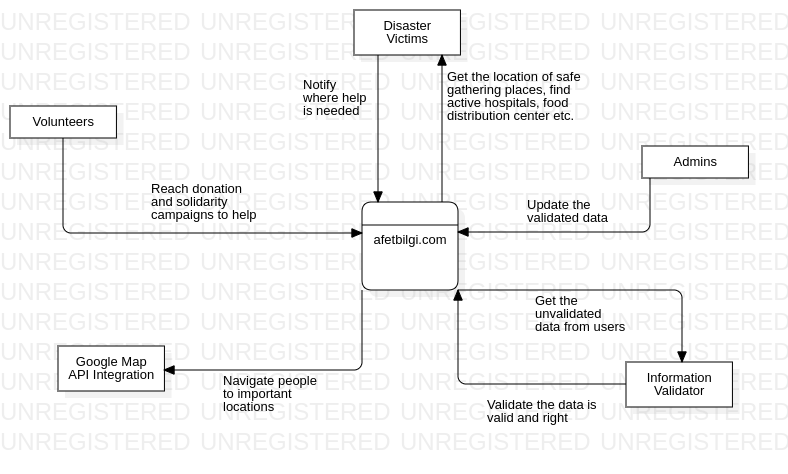
\includegraphics[scale = 0.60]{assets/SystemContextDiagram.png}
        \caption[System Context Diagram]{System Context Diagram for afetbilgi.com}
    \end{center}
\end{figure}

\subsubsection{System Interfaces}

\begin{itemize}
    \item \textbf{Google Maps API: } Afetbilgi.com uses Google Maps API to navigate people to locations which is on the website to the user. This system shows users to where they are, close evacuation points, emergency gathering areas, temporary accomamodation places, food distribution centers, gas stations, active hospitals and pharmacies. By this integration, in the emergency cases, people can find where and how to go rapidly. Thus, it may increase the survival rate in vital situations. 
    \item \textbf{Database Management Interfaces: } Authorized person validate the informations by teams. Afetbilgi.com admins updates the database with the validated information thanks to the validation teams and volunteers. With this mobilization, this system works with accuracy, speed, and simplicity principles. It also prevent disinformation. In addition to that, by the city filtering system, users can reach only the needed information in emergency situations. 
    \item \textbf{PDF Integration: } This system allows users that they can download the crucial information for the city they need since the communication and network systems may get damage and it may not reachable. Therefore, by downloading only the crucial information may increase the speed of help.
    \item \textbf{Multi Language Support: } This system allows afetbilgi.com reach the broader effect on the disaster situation. Foreigners in the area can reach the system more easily.
\end{itemize}

\subsubsection{User Interfaces}

Users can use this application by using their internet browsers. When they reach the website users can see that one of the features of the website is simplicity. All the submenu's and filters are clear and simple. The backend and frontend of the website is lightweight; therefore, in the disaster area users can reach the website with the slow internet speeds. 

\begin{figure}[H]
    \begin{center}
        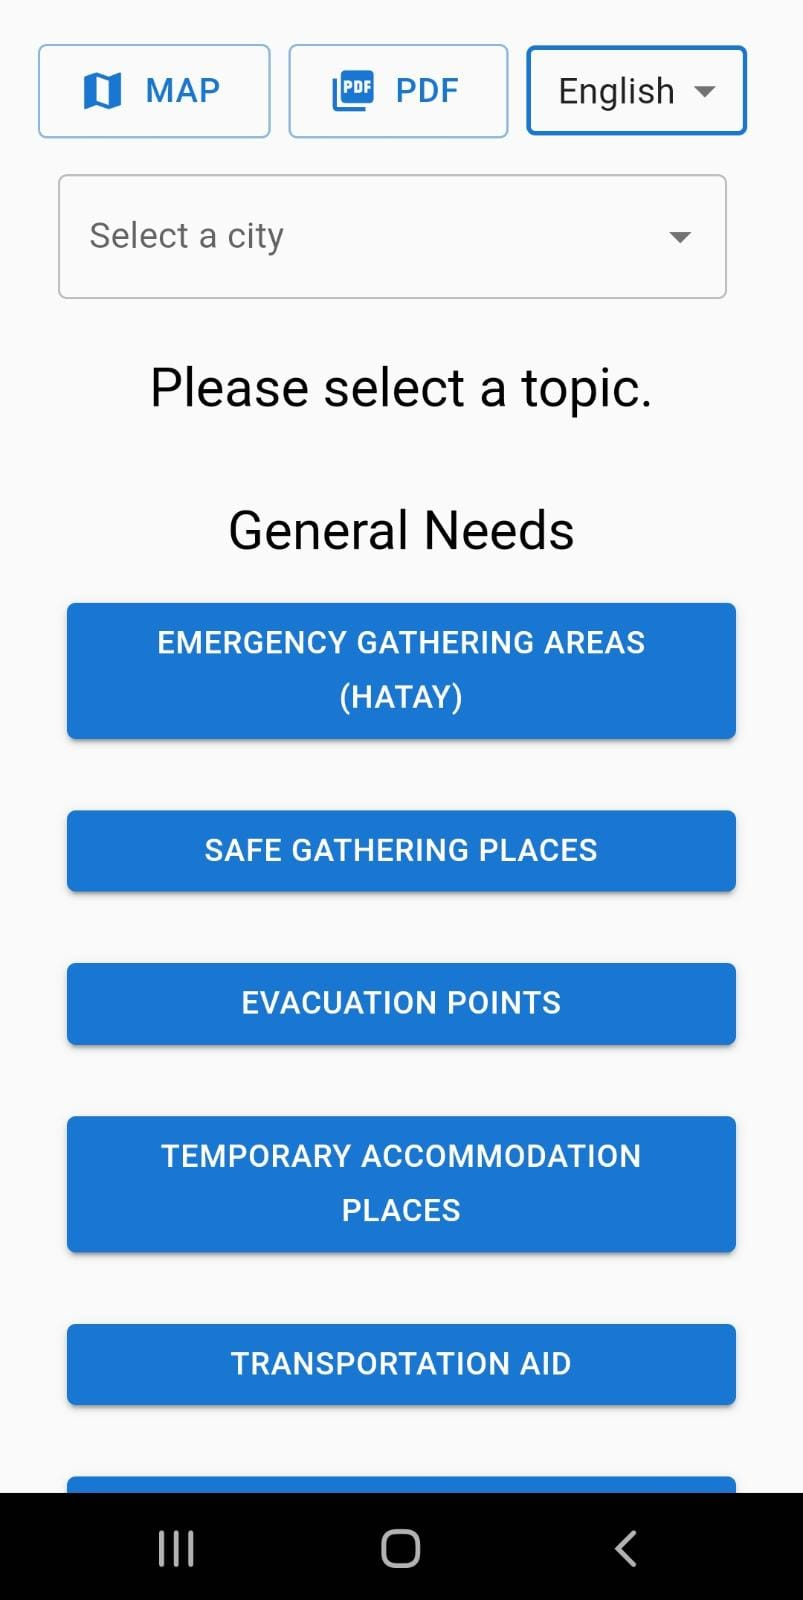
\includegraphics[scale = 0.10]{assets/mainmenu.jpeg}
        \caption[Main Menu in Mobile Devices]{Main Menu in Mobile Devices of afetbilgi.com}
    \end{center}
\end{figure}

\begin{figure}[H]
    \begin{center}
        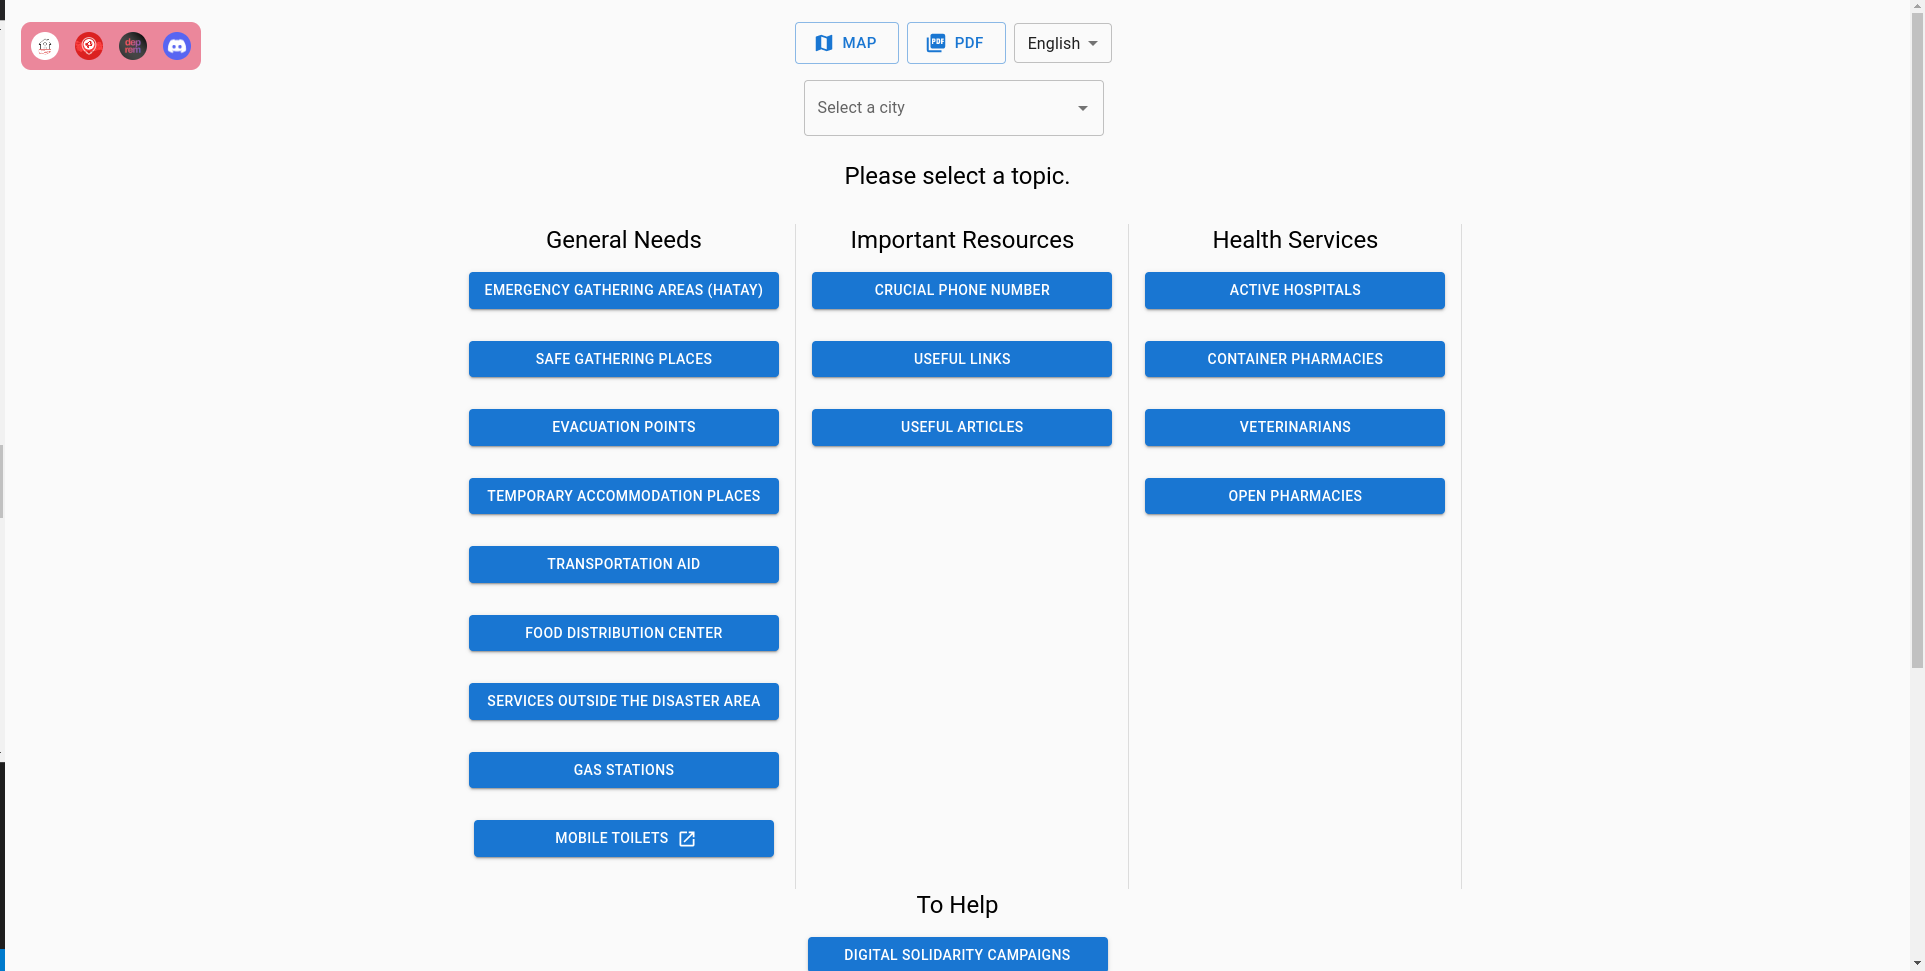
\includegraphics[scale = 0.18]{assets/desktopInterface.png}
        \caption[Main Menu in Desktop]{Main Menu in Desktop of afetbilgi.com}
    \end{center}
\end{figure}

With the Google Maps API integration, users can see their exact locations. In addition to that, they will find the important locations which they are close to them. Also by the filtering setting, it increases the practicality and becomes task oriented system. When the user select the desired locations, the website redirect them to google maps navigation system. 

\begin{figure}[H]
    \begin{center}
        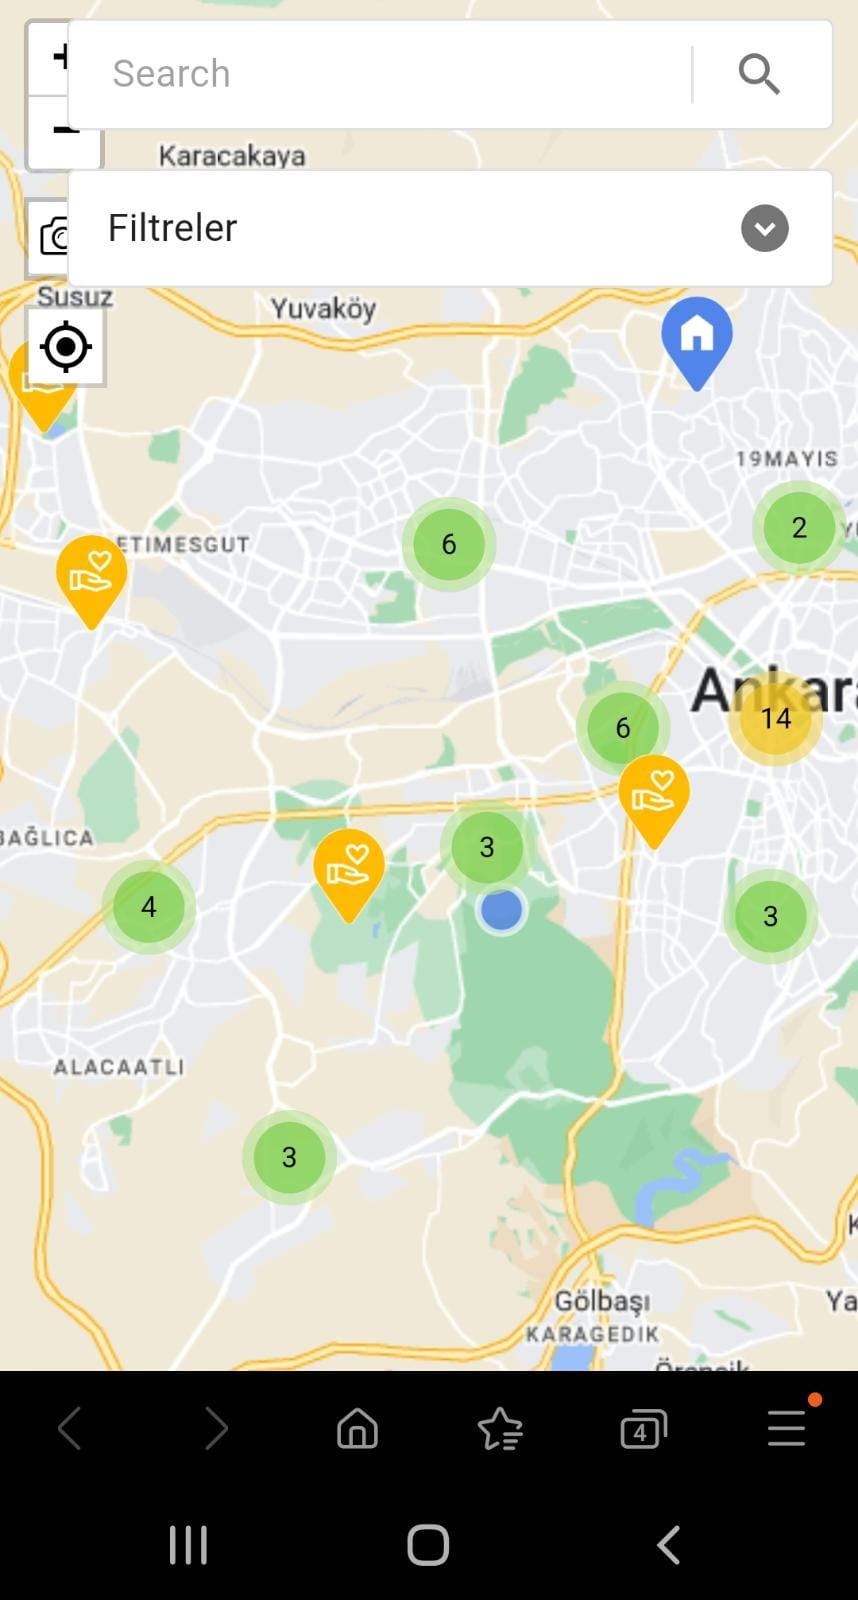
\includegraphics[scale = 0.15]{assets/maps.jpeg}
        \caption[Maps Integraion]{Maps Integration}
    \end{center}
\end{figure}

\begin{figure}[H]
    \begin{center}
        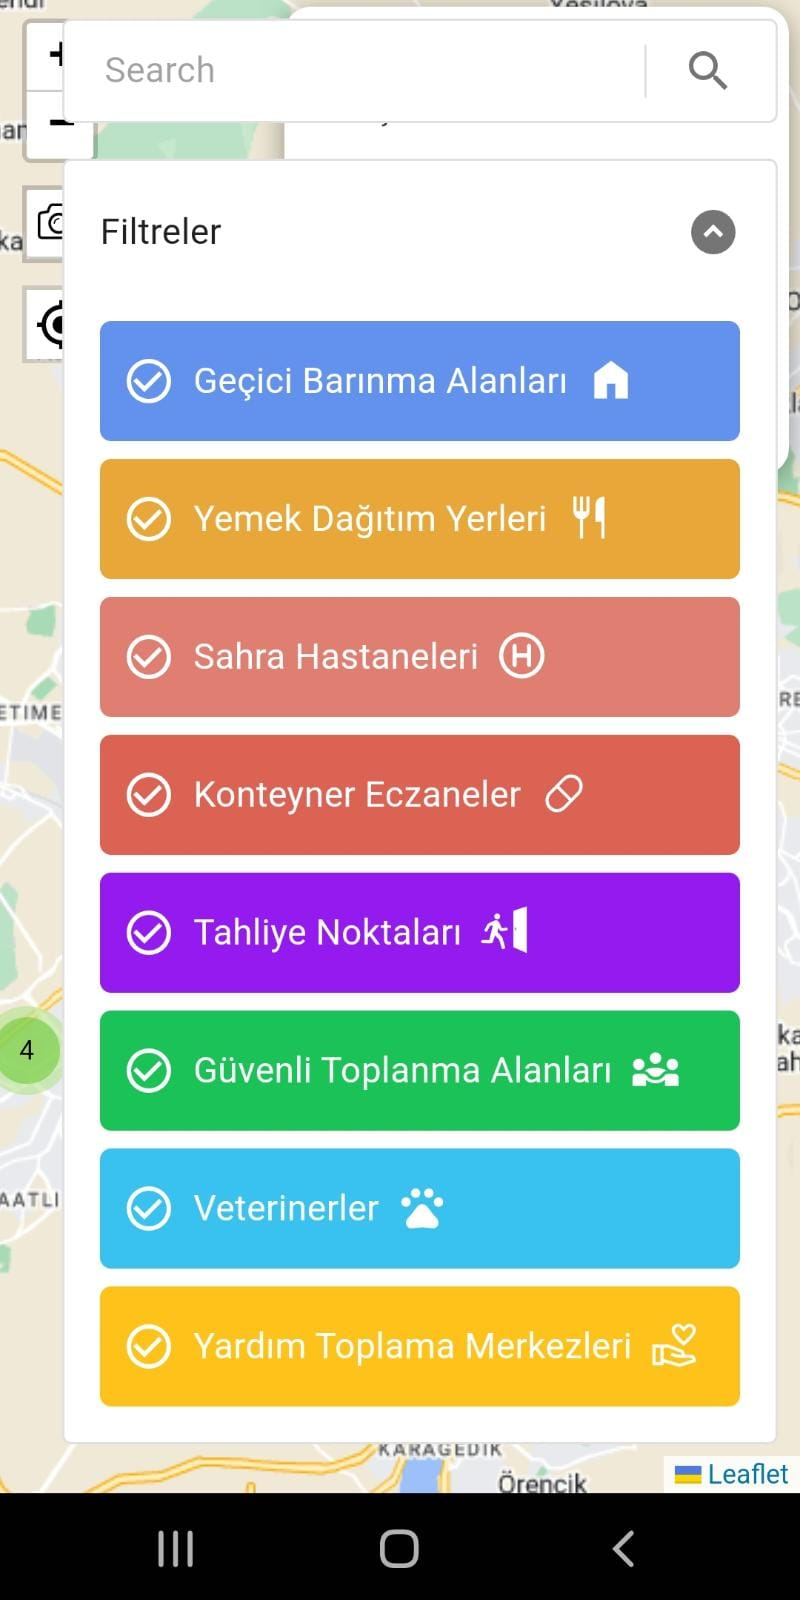
\includegraphics[scale = 0.15]{assets/filter.jpeg}
        \caption[Filter Settings for Map]{Filter Settings for Map}
    \end{center}
\end{figure}



\begin{figure}[H]
    \begin{center}
        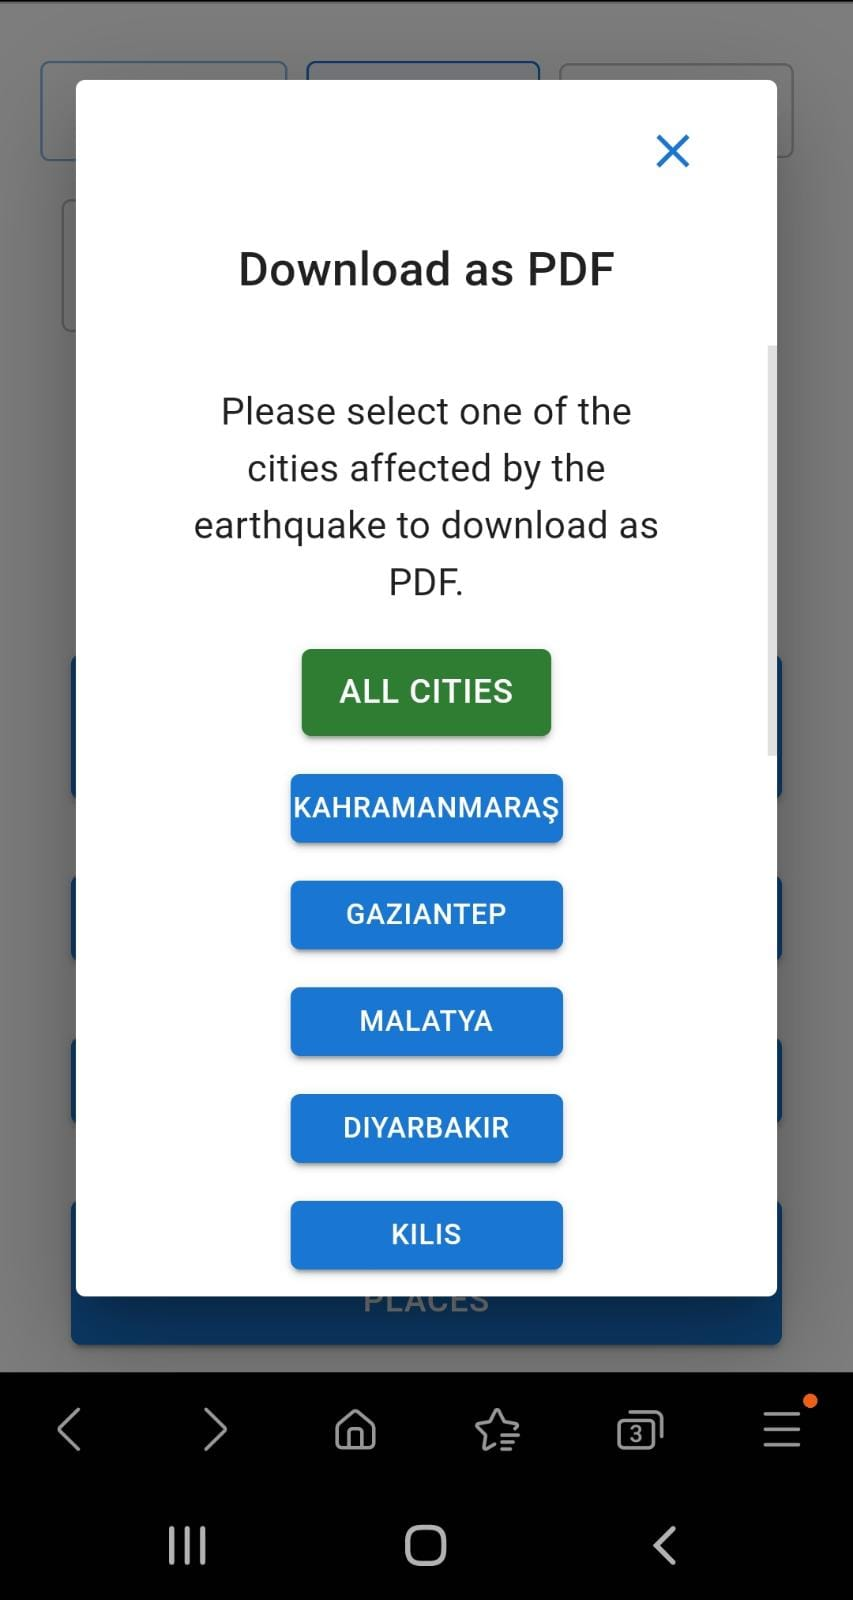
\includegraphics[scale = 0.15]{assets/pdf.jpeg}
        \caption[PDF Download Menu]{PDF Download Menu by Selecting Cities}
    \end{center}
\end{figure}

\begin{figure}[H]
    \begin{center}
        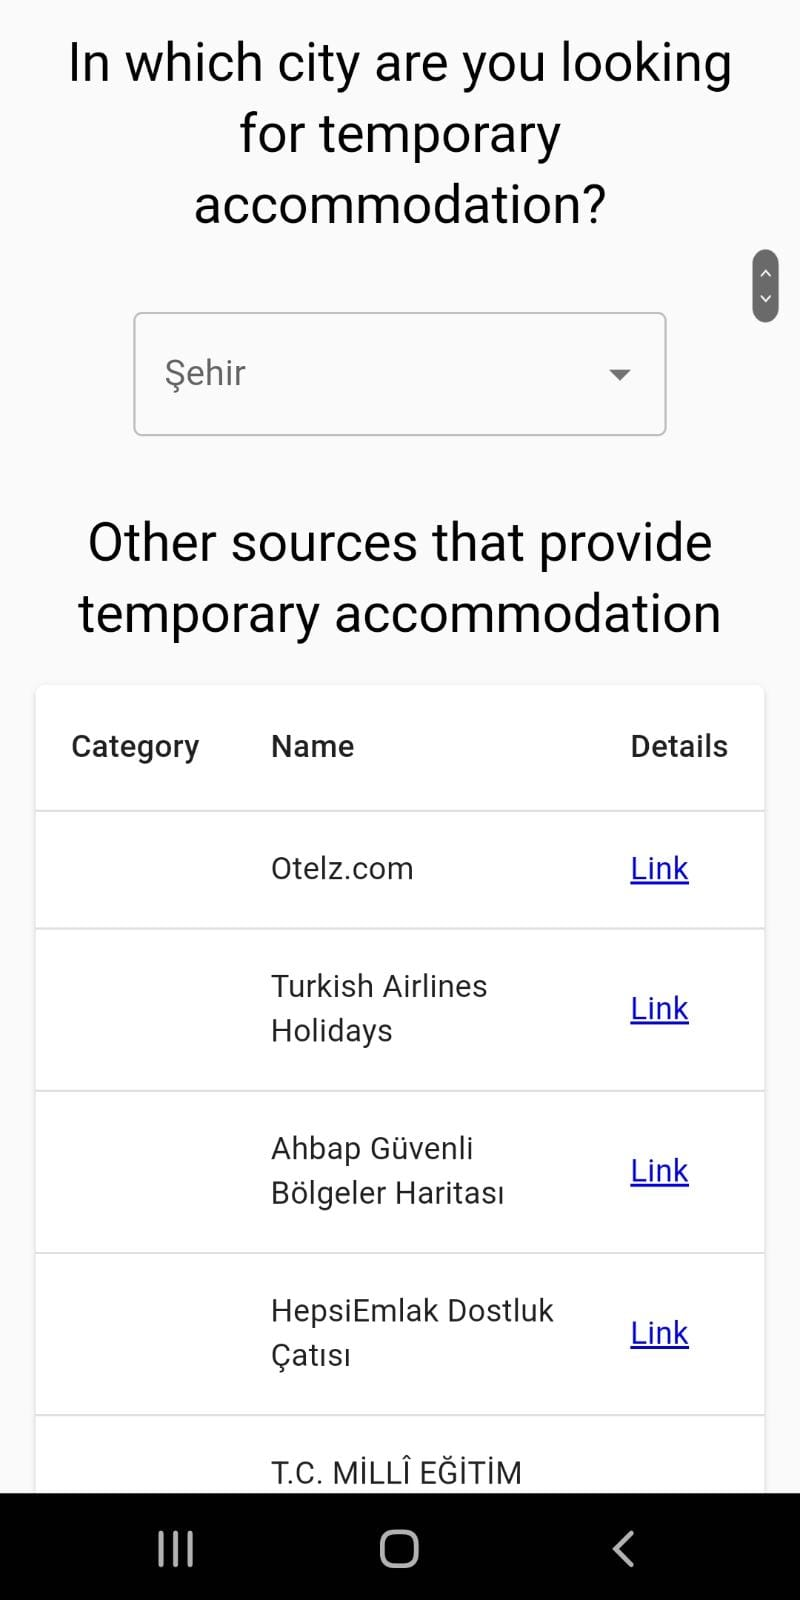
\includegraphics[scale = 0.15]{assets/accommodation.jpeg}
        \caption[Accommodation Menu]{Accommodation Menu}
    \end{center}
\end{figure}

\begin{figure}[H]
    \begin{center}
        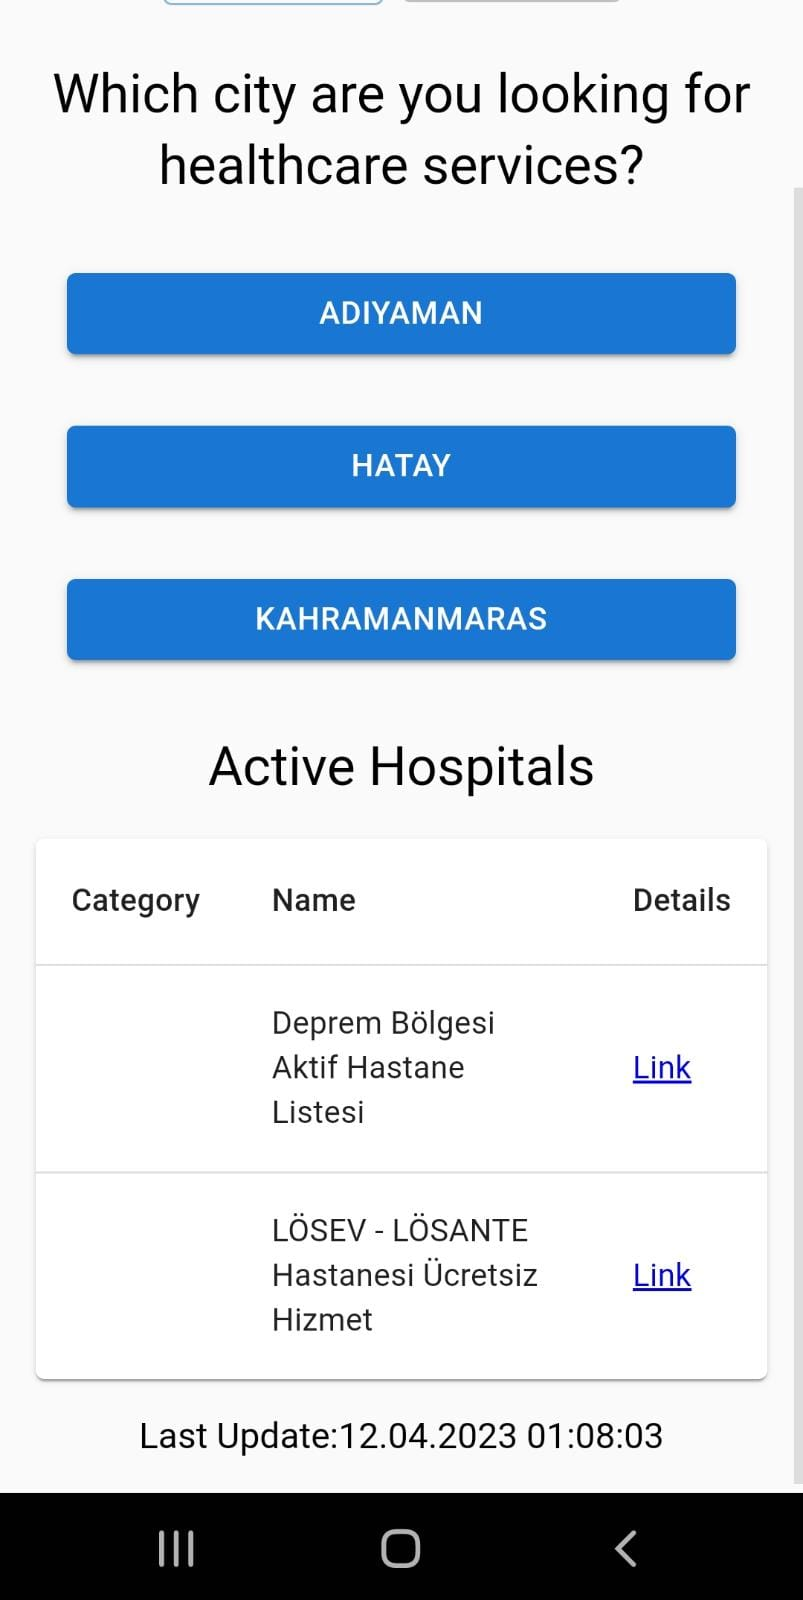
\includegraphics[scale = 0.15]{assets/healthcareinterface.jpeg}
        \caption[Healthcare Services Menu]{Healthcare Services Menu}
    \end{center}
\end{figure}

\subsubsection{Hardware Interfaces}

The system requires device which has an internet access. If the user want to use Google Maps API it should also have an gps in its device.

\subsubsection{Software Interfaces}

\begin{itemize}
    \item \textbf{Database: } The system uses JSON file to store the data. This system does not require an complicated database system.
    \item \textbf{Operating Systems: } The system can reachable by any device which has an internet browser and access.
    \item \textbf{Google Maps: } The system use Google Maps to show the important locations and where the user are in the map and allow them to reach them.
\end{itemize}

\subsubsection{Memory Constraints}

There is not an issue about memory constraints in the system. System should have enough memory to hold necessity information however, it requires a very low memory which can sustainable easily. 

\subsubsection{Operations}

The operations provided by afetbilgi.com can be partitioned into: \\

\textbf{User operations: }

\begin{itemize}
    \item 
\end{itemize}

\textbf{Admin operations: }
\begin{itemize}
    \item 
\end{itemize}



\subsection{System Functions}

\subsection{Stakeholder Characteristics}

\subsection{Limitations}

\section{Definitions}